\section{abstract}
Predicting the rate of nonfacilitated permeation of solutes across lipid bilayers is important to drug design, toxicology, and signaling. These rates can be estimated using molecular dynamics simulations combined with the inhomogeneous solubility-diffusion model, which requires calculation of the potential of mean force and position-dependent diffusivity of the solute along the transmembrane axis. In this paper, we assess the efficiency and accuracy of several methods for the calculation of the permeability of a model DMPC bilayer to urea, benzoic acid, and codeine. We compare umbrella sampling, replica exchange umbrella sampling, adaptive biasing forces, and multiple-walker adaptive biasing forces for the calculation of the transmembrane PMF. No definitive advantage for any of these methods in their ability to predict the permeability coefficient \perm~was found, provided that a sufficiently long equilibration is performed. For diffusivities, a Bayesian inference method was compared to a Generalized Langevin method, both being sensitive to chosen parameters and the slow relaxation of membrane defects.
%{\bf Although the performance for predicting log Pm was generally fair, the accuracy of these calculations could be improved by the development of more accurate force fields and methods for the calculation of the PMF and diffusion coefficient profiles.}
Agreement within 1.5 log units of the computed \perm~with experiment is found for all permeants and methods.  Remaining discrepancies can likely be attributed to limitations of the force field as well as slowly relaxing collective movements within the lipid environment.  Numerical calculations based on model profiles show that \perm~can be reliably estimated from only a few data points, leading to recommendations for calculating \perm~from simulations.

% suggestion from Chris C.:
%Although the agreement with experiment, however perfectible, is by and large reasonable, the present set of calculations brings to light aspects where improvement is desirable. While the methodology is robust and has proven appropriate for a variety of applications, sampling remains a major concern, in particular for the estimation of diffusivities, owing to the slowly relaxing collective movements within the lipid environment. The discrepancies between theory and experiment also illustrate the shortcomings of macromolecular force fields in describing small, drug-like permeants.

%YW: replacing the last sentence with something on concentrating the computing resources on a few data points? sth like: Our analysis also shows that only a few data points on the PMF and diffusivity profiles contribute significantly to Pm. For this reason, we recommend focusing computational resources on these critical points, rather than evenly spreading them over the entire transmembrane axis.

%!TEX ROOT = ../ctl-phd-thesis.tex

\par The goal of biology is to understand life to an extent that one can predict the eventual behaviors of a living system under or in the absence of a stimulus or perturbation.
Although many debate the utility of quantitative modeling in answering this question, I will abstain from such discussion and focus on the benefits of modeling as I view them.
The development of a whole cell or organism model has become a hot topic in modern biology\cite{Roberts2014}.
As biologists uncover the mysteries which make life possible, they unveil new complexities\cite{CheckHayden2010}.
These complex and non-linear behaviors are not amenable to scrutiny via traditional research methods which are driven by classical hypotheses (i.e., by varying one parameter at a time and observing and characterizing the results to form conclusions).
Simple experimental models, while elegant, test isolated model behaviors in simplified systems which are often not generalizable.
In order to derive a general conclusion, many expensive experiments must be run to explore the solution space at large potential cost.

\par One strategy to reduce the experimental cost burden is to shift towards inexpensive mathematical modeling.
Mathematical models in biology are increasing in popularity, and come in a wide variety of flavors\cite{Gunawardena2014}.
For example, there are information and data driven models as well as models based on the fundamentals of physical principles.
In this dissertation, I will focus on the development of methods in support of the latter.
By codifying our knowledge of the physical world into a model, we can gain many benefits.
First, physical models can serve as a glue to reconcile the results of individual experiments under isolated conditions.
Cleverly designed mathematical models are also amenable to computed solutions using numerical methods.
Combining knowledge and computation, inexpensive parameter sweeps that eliminate physical impossibilities and guide experimental efforts can serve to reduce the experimental cost of biology.

\par Physical models can also produce other benefits for science.
During the design and validation phase of model construction, when a physical model fails to reproduce experimental results, this is a litmus test for the limitations of our current understanding.
By studying the assumptions of the model and querying the differences between prediction and experiment, scientists can pinpoint possible knowledge gaps.
Once a physical model is sufficiently validated, due to the fundamental basis of transferable physical properties, the models can also be used to generate prospective predictions.
For example, in an inspiring study, Hodgkin and Huxley created a famous model describing the propagation of an action potential along a giant squid axon\cite{HUXLEY1952}.
Although the model was based on empirical fitting of electrophysiology data, many speculated upon the physical implications of the mathematics.
One term in particular, predicting the presence of four voltage-sensitive gates in the sodium ion channel, was later experimentally confirmed by crystallographic structure which resolved the tetrameric channel structure\cite{Sigg2014a}.

\par We live in an exciting time, where there is a convergence of emerging structural data, legacy experimental parameters, and computational power.
In order to understand life, we must embrace the complexity of biology.
The work described in this dissertation seeks to address several challenges which hinder the routine application of large systems biology models.
This includes the computational prediction of various biological rates such as diffusion, permeability, and binding/unbinding, strategies to develop models of individual protein dynamics, and the capacity to generate multiscale geometric models suitable for biological modeling.

\section{Overview of Chapter Contents}

\par To reiterate and highlight the opportune convergence of computing and biological data, \cref{chap:exascale} discusses the potential applications and gains afforded by future exascale supercomputers to biology.
This chapter provides some perspective on the role that computers can play to solve various biological problems.
We speculate upon not only the contributions of computation to basic science, but also upon the impact of computation and technology on translational fields such as personalized medicine.
In this chapter, we also address and frame some of the aforementioned challenges to future modeling efforts with solutions described in the subsequent chapters.

\par Owing to the complexity of biology, a complete systems model will require the definition of many rates.
Due to the basic nature of many of these measurements, the experimental work to measure these values may not be publishable and is therefore difficult to source.
Although robotics which automate assay development and screening are amenable to some tasks, the complexity of experimental setups for measuring kinetic properties can often hinder accurate and high-throughput measurement.
To augment the existing data and measurements, molecular simulations such as Molecular Dynamics (MD) can be employed to generate estimates\cite{Leach2001,Durrant2011a}.
MD effectively integrates the classical equations of motion for an atomistic system.
Given that the typical timescales of simulation are typically much shorter than the timescales of the process of interest, brute force MD simulations can rarely capture the dynamics of interest with sufficient statistics.
Instead, using strategies derived from statistical mechanics, many enhanced sampling strategies have been developed to facilitate the estimation of classically intractable properties\cite{Chipot2007,Tuckerman2010}.
In \cref{chap:permeability}, we compare the efficiency of four enhanced sampling strategies to compute drug passive membrane permeability.
We find that there are many orthogonal degrees of freedom which can hinder the convergence of these calculations and recommend some best practices for future work.

\par While studying membrane permeability, I had many stimulating discussions with my colleague Lane Votapka on the topic.
During our overlap in the group, Lane was working on the development of a software tool which facilitates the use of milestoning to compute various rates.
Milestoning is another enhanced sampling strategy where, instead of observing the full transition from start to finish of a process, we collect statistics of transitions along many small segments of the full pathway and stitch them together in postprocessing\cite{Faradjian2004,Majek2010,Vanden-Eijnden2008,Kirmizialtin2011,Votapka2015,Bello-Rivas2015,Votapka2017c}.
The application of milestoning theory to permeability calculations was not straightforward since the natural currency of milestoning is transition probabilities, while the expressions to compute permeability required potentials of mean force.
To solve this, Lane derived a new relation to compute permeability values using transition probabilities from milestoning which we validated using a toy model inspired by my prior work on permeability.
This research is described in \cref{chap:mileperm}.

\par After learning about the virtues of the milestoning method, the group started thinking about possible applications of milestoning to compute other rates of interest.
By chance, my colleague Ben Jagger and I met Professor Chia-en Chang at a local conference where she was presenting preliminary results describing brute-force MD calculations of host-guest binding kinetics and thermodynamics\cite{Tang2017}.
This dataset which contained several ligands, experimentally determined kinetics, and brute-force MD was the ideal system to benchmark the use of SEEKR\cite{Votapka2017c}.
Chia-en kindly shared the dataset with us and working with Ben, we predicted the binding kinetics of the system using milestoning.
The results of this work are described in \cref{chap:bcd} along with some best practices to monitor the convergence of computed rate estimates which we developed along the way.

\par Also of interest for biological simulations is the dynamics of protein movement.
Not only are the dynamics of proteins critical to their biological function, but protein dynamics also influence phenomena such as drug binding.
In \cref{chap:allostery}, we present a review of many different strategies to use computers to inform the rational design of allosteric drugs.
Previously I had worked with Robert Malmstrom on a paper describing the applications of Markov state models to model protein kinase A dynamics with and without cyclic AMP\cite{Malmstrom2015a}.
During this project, we started thinking about the use of MSMs to model perturbations to the conformational ensembles of protein targets by drugs and using the information to support drug discovery efforts.
Later working with Bryn Taylor, we investigated the impact of drug binding to GPCR CCR2.
The generation and description of our CCR2 MSMs is presented in \cref{chap:ccr2}.

\par Another important aspect of cell modeling is the generation of computable geometries to represent cellular scenes.
Meshes are commonly used in engineering fields as a general geometric representation.
The use of meshes is desirable since they are often also compatible with simulation methods such as finite elements.
However, the numerical behavior of algorithms is often limited by mesh conditioning.
To support the development of robust mesh generation codes for biological geometries, working with John Moody, we developed the Colored Abstract Simplicial Complex library which is described in \cref{chap:asc}.

\par In summary, the work in this dissertation explores the use of various modeling strategies to predict values of interest or to generate geometric meshes in support of future multiscale modeling efforts.


%Results
%  *rationale for the choice of permeants (Yi, Nelson, Chris T.)
%    -range of expected logPs, experimental data for real membranes (not just PAMPA)
%    -also explores force field reliability (codeine just run through paramchem for example)

\section*{Results and Discussion}
Below, we report the membrane permeability coefficients (\perm) of urea, benzoic acid, and codeine computed with four different methods, namely, US, REUS, ABF and MW-ABF.  We also present a detailed analysis of two methods for the computation of diffusivity, namely, a Bayesian inference method and a Generalized Langevin method. While we did not test metadynamics, another common free-energy method, it has recently been favorably compared with US for water-membrane partitioning, nonetheless while suffering the same shortcomings~\cite{Bochicchio2015}.  Initial states, i.e., positions of the permeant within the bilayer, were generated using 100-ns steered MD simulations~\cite{Izrailev1997,Sotomayor2007} in which the permeant is pulled from one side of the membrane to the other (see Methods).
%We will first compare our results with experimentally measured logP$_{m}$, and then evaluate the performance of different methods in computing the PMFs and diffusivities of various permeants, followed by a discussion on the error and robustness of the four methods.

The three permeants studied here, shown in Fig.~\ref{fig:permeants}, are chosen for their diverse chemical properties:
their molecular weights range from 60\,g/mol (urea) to 299\,g/mol (codeine);
their hydrophilicity, as measured by the octanol:water partition coefficient, differs by over two orders of magnitude;
and most importantly, the experimentally determined \perm~of the three permeants span five orders of magnitude (Table\,1), making them a relatively robust test set for \perm~calculation via different methods. Of the three permeants, benzoic acid is the only permeant that exhibits a formal charge at pH=7. Nonetheless, only its neutral form is considered in our calculation. This treatment is consistent with the corresponding experimental protocol~\cite{Walter1984}, where fluxes at several pH values are measured to determine the `intrinsic permeability' corresponding to the un-ionized form of a given molecule. The underlying assumption of such a protocol, i.e., only the non-ionized form of benzoic acid contributes significantly to \perm, has been confirmed experimentally~\cite{Walter1984}.

\begin{figure}[htbp]
\begin{center}
	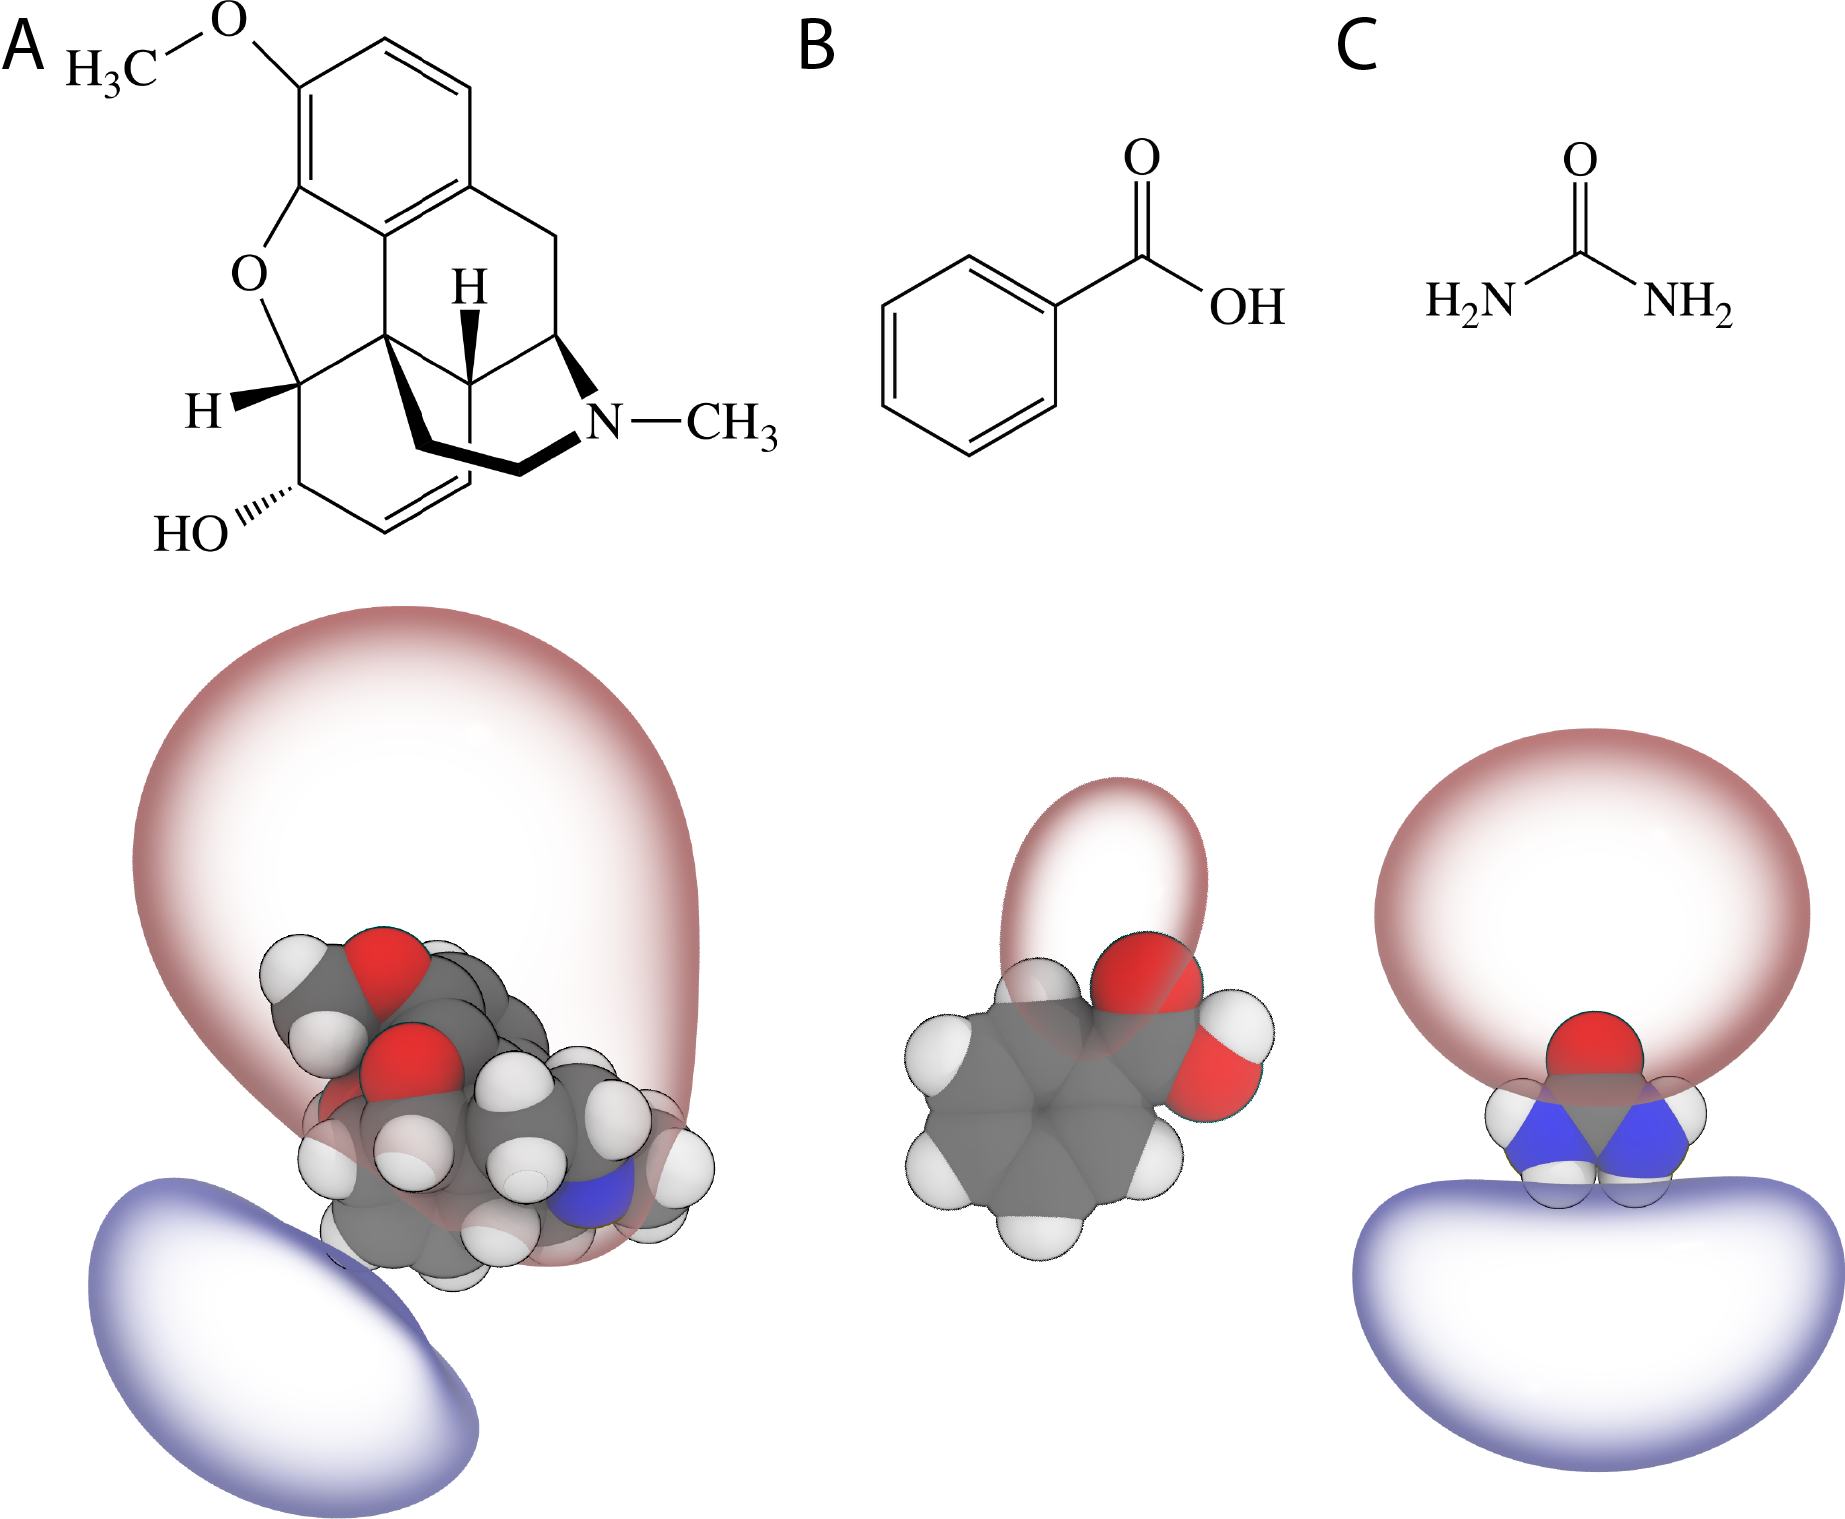
\includegraphics[width=0.6\textwidth]{2015-permeability/Figures/permeants1}
	\caption{Three permeants tested shown as 2D schematics (top) and 3D structures rendered with the $\pm 5$ kT/e electrostatic potential isosurfaces
% JC: What is PME?
% calculated by PME
using the assigned CGenFF charges (bottom).  (A) codeine.  (B) Benzoic acid (neutral).  (C) Urea.}
	\label{fig:permeants}
\end{center}
\end{figure}

%We should add a section about system set up, to include a description of the use of SMD to generate the starting states. This brief section could go here.
% whoops, overlooked this comment; still SMD is now mentioned above

%    Section: "Calculated permeabilities" (Yi, Nelson, Chris T.)
%      -the final, BEST logPs from each method at ~1-1.4 us each (Table 1)
%      -plots showing the comparison 
%      -what are the errors?  (just numerically at this point) 
%      -does increasing simulation time help?  (not really: case of urea)

\subsection*{Computed vs. experimental \perm}
  \par The computed log\perm~of the three permeants are listed in Table 1, along with the corresponding experimental references obtained from egg phosphatidylcholine bilayers (urea~\cite{Gallucci1971}, codeine~\cite{Orbach1980} and  benzoic acid~\cite{Walter1984}). 
  % Egg lecithin and egg-PC are interchangeable. Both papers purchased egg-PC from avanti inc among other sources.
  From Table~1, it is clear that the majority of computed \perm~values exceed the corresponding experimental data by 1--2 orders of magnitude. For comparison, we define $\Delta$log\perm = log\permcom - log\permexp, where log\permcom~and log\permexp~are the computed and experimental log\perm, respectively. Negative $\Delta$log\perm~values are only observed for urea, the most hydrophilic of the three permeants.  Results obtained with different methods also show the largest discrepancy for urea: the US and REUS  methods underestimate log\perm~by 0.87 and 0.51, whereas ABF and MW-ABF overestimate it by 0.71 and 1.14, respectively. For benzoic acid and codeine, all the methods overestimate log\perm~by 0.71 to 1.67. 

  %%\documentclass[11pt,letterpaper]{article}

%%\usepackage{color}

%%\setlength{\textwidth}{17cm}
%%\setlength{\textheight}{20.5cm}
%%\setlength{\oddsidemargin}{-.1cm}
%%\setlength{\topmargin}{-2 cm}

%%\renewcommand{\baselinestretch}{1.0}

%%\newcommand{\hl}[1]{\textcolor{red}{#1}}
\newcommand{\hl}[1]{\textbf{#1}}
\providecommand{\e}[1]{\ensuremath{\times 10^{#1}}}

%%\begin{document}

\begin{table}[h]
\centering
%\resizebox{\textwidth}{!}
{
\begin{tabular}{|c|c|c|c|}
\hline
 & Urea & Benzoic Acid & Codeine     \\ \hline 
%PAMPA  & \multicolumn{2}{c|}{-9.0}          & \multicolumn{2}{c|}{-3.94}                                                  & \multicolumn{2}{c|}{xx}        \\ \hline
% multiple columns probably too confusing - graph shows time dependence better anyway
% & \multicolumn{2}{c|}{Urea} & \multicolumn{2}{c|}{Benzoic Acid} & \multicolumn{2}{c|}{Codeine}      \\ \hline 
%Experiment & \multicolumn{2}{c|}{-5.4}          & \multicolumn{2}{c|}{-0.26}                                                  & \multicolumn{2}{c|}{-0.85}        \\ \hline
%US                & -5.97 (1.1\,$\mu$s)    & -6.27 (2.9\,$\mu$s)   & 0.35 (1.1\,$\mu$s)                         & 0.45 (1.4\,$\mu$s)                         & 0.08 (1.1\,$\mu$s)     & 0.03 (1.4\,$\mu$s)   \\ \hline
%RE-US              & -5.28 (1.1\,$\mu$s)    & -5.91 (4.3\,$\mu$s)   & 1.11 (1.1\,$\mu$s)                         & 1.17 (1.4\,$\mu$s)                         & 0.67 (1.1\,$\mu$s)     & 0.64 (1.4\,$\mu$s)   \\ \hline
%ABF               & \multicolumn{2}{c|}{-4.69 (0.9\,$\mu$s)} & \multicolumn{2}{c|}{1.16 (0.9\,$\mu$s)}                                           & 0.59 (1.1\,$\mu$s)     & 0.82 (2.7\,$\mu$s)   \\ \hline
Experiment & -5.4          & -0.26                                             & -0.85      \\ \hline
US                & -6.27 (2.8\,$\mu$s)   & 0.45 (1.4\,$\mu$s)             & 0.03 (1.4\,$\mu$s)   \\ \hline
REUS              &  -5.91 (4.3\,$\mu$s)   & 1.17 (1.4\,$\mu$s)   & 0.64 (1.4\,$\mu$s)   \\ \hline
ABF               & -4.69 (0.9\,$\mu$s) & 1.16 (0.9\,$\mu$s)      &  0.82 (2.7\,$\mu$s)   \\ \hline
% from JC: these are the numbers I get with the new Dz
%ABF               & \multicolumn{2}{c|}{-4.65 (0.9\,$\mu$s)} & \multicolumn{2}{c|}{1.14 (0.9\,$\mu$s)}                                           & 0.51 (0.9\,$\mu$s)     & 0.68 (2.7\,$\mu$s)   \\ \hline
%ABF               & \multicolumn{2}{c|}{-5.04 (0.9\,$\mu$s)} & \multicolumn{2}{c|}{0.41 (0.9\,$\mu$s)}                                           & -0.14 (0.9\,$\mu$s)     & -0.06 (2.7\,$\mu$s)   \\ \hline
% the following is from Jeff
MW-ABF    &  -4.26 (1.4\,$\mu$s)   & 0.81 (0.7\,$\mu$s)       & 0.18 (1.1\,$\mu$s) \\ \hline
%MW ABF    & -4.19 (1.1\,$\mu$s)    & -4.21 (1.4\,$\mu$s)   & \multicolumn{2}{c|}{0.79 (0.7\,$\mu$s)}                                           & \multicolumn{2}{c|}{0.19 (1.1\,$\mu$s)} \\ \hline
%MW ABF (2ps)    & -3.43 (1.1\,$\mu$s)    & -3.45 (1.4\,$\mu$s)   & \multicolumn{2}{c|}{1.45 (0.7\,$\mu$s)}                                           & \multicolumn{2}{c|}{0.88 (1.1\,$\mu$s)} \\ \hline
%MW ABF (8ps)    & -3.84 (1.1\,$\mu$s)    & -3.86 (1.4\,$\mu$s)   & \multicolumn{2}{c|}{1.14 (0.7\,$\mu$s)}                                           & \multicolumn{2}{c|}{0.55 (1.1\,$\mu$s)} \\ \hline
\end{tabular}
}
\caption{ log\perm~of the three permeants examined in this study. The unit of \perm~is cm/s. Experimental values are obtained from \citenum{Orbach1980}, \citenum{Gallucci1971} and \citenum{Walter1984}. 
For each computed log\perm, the length of the simulation used in the computation is shown in parenthesis.}
\label{table:results}
\end{table}

%%\end{document}



  Fig.~\ref{fig:deltaP} also reveals that with the possible exception of urea, increasing simulation time does not significantly improve agreement with experiment.  Even for urea, the computed \perm~tends to plateau once the total simulation time exceeds 1\,$\mu$s.  It is unlikely that \perm~has converged, however, but requires much longer time scales (milliseconds) to sample very slow membrane reorganization processes~\cite{Neale2011}.  
      
%  Nonetheless, it is of considerable value to examine why shorter simulations manage to produce similar results as longer ones. As discussed in the following section, the symmetrization and cyclization of the computed free energy profiles likely play a part in this process. 

  \begin{figure}
    \centering
    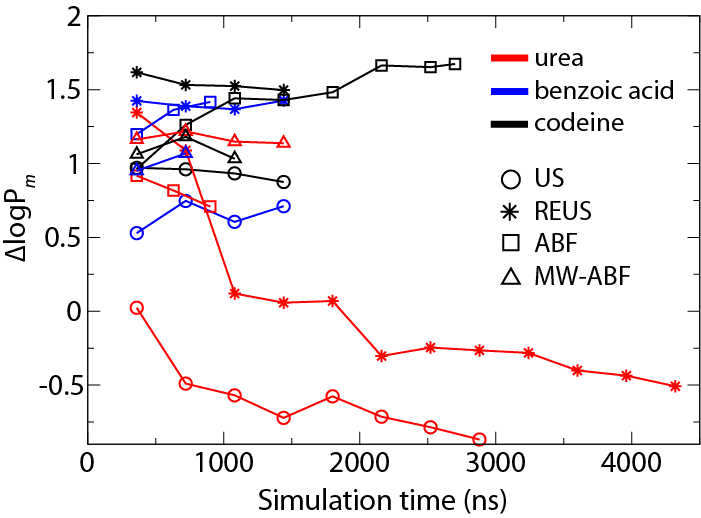
\includegraphics[width=0.65\textwidth]{Figures/dlogP-recolor.png}
    \caption{ $\Delta$log\perm~of urea (red), benzoic acid (blue) and codeine (black) as a function of simulation time. %For each permeant, $\Delta$log\perm = log\permcom - log\permexp, where log\permcom~and log\permexp~are the computed and experimentally measured log\perm~values, respectively. 
    Results obtained with different methods are indicated using the following symbols: US (circle), REUS (star), ABF (square), MW-ABF (triangle). }
    \label{fig:deltaP}
  \end{figure}

%   Section: "PMFs"  (JC & Conner)
%      -notable asymmetry across the membrane center (focus on urea)
%      -effect of making the US PMFs symmetric using g_wham, along with autocorrelation time estimates
%      -longer equilibration makes US converge more quickly
%      -comparison using data from z = (0,36) @ 20 ns/window vs. z = (-36,36) @ 10 ns/window

\subsection{Potentials of Mean Force}
  \par In the solubility-diffusion model, the PMF is a critical component of the permeability (see Eq.~\ref{eq:solubility-diffusion}).  Given its exponential weighting, the PMF may even be considered the greatest contributor to the permeability, making its accurate calculation of paramount importance.  To determine the best approach for calculating the PMF, we have compared four methods mentioned earlier and investigated the appropriate balance between equilibration time and sampling time.

\begin{figure}[htbp]
\begin{center}
	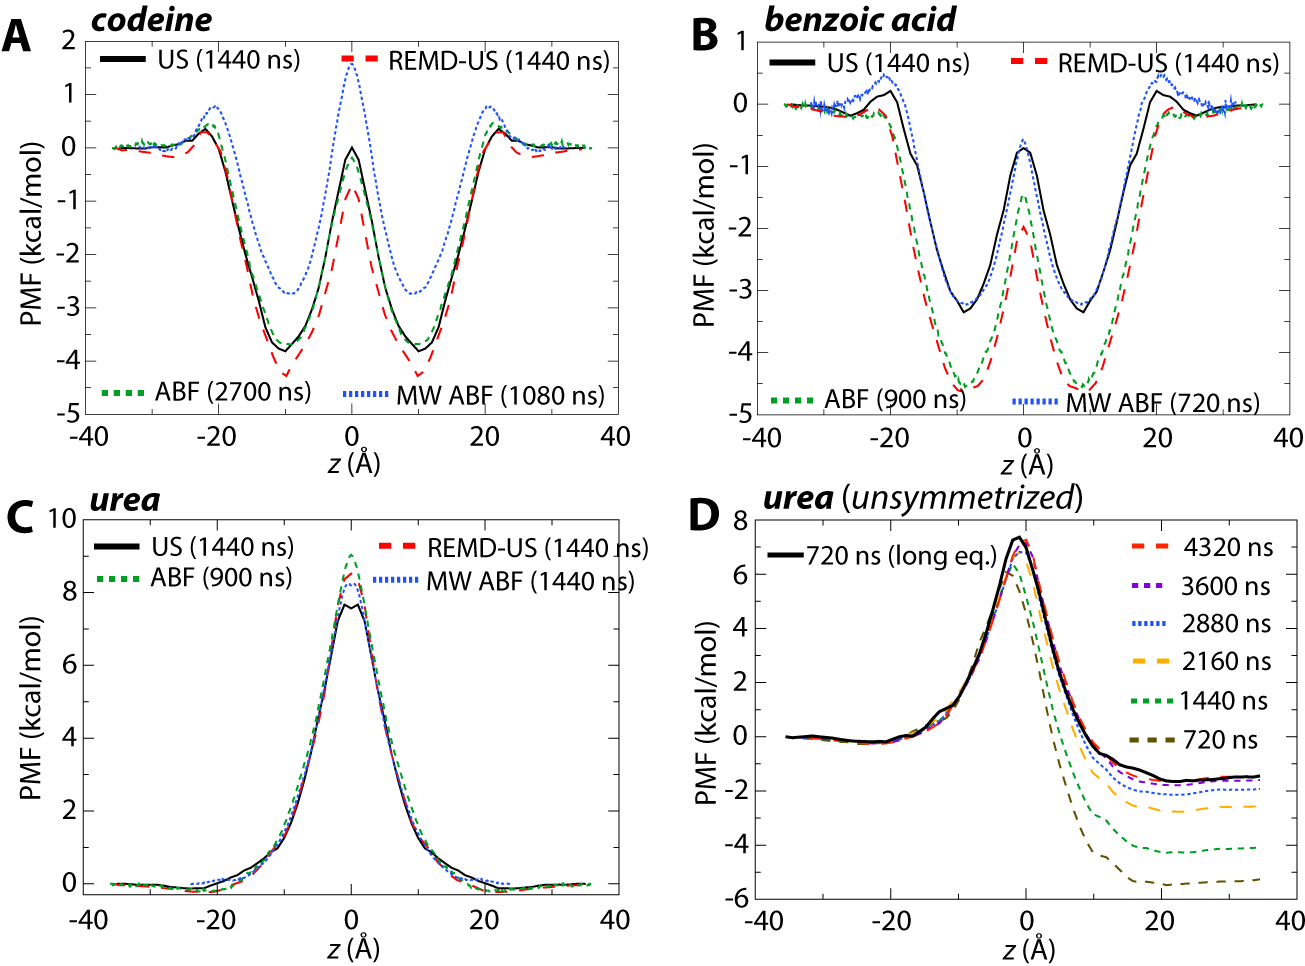
\includegraphics[width=0.8\textwidth]{Figures/PMFs-all}
	\caption{Potentials of Mean Force (PMFs) for the permeants (A) codeine, (B) benzoic acid, and (C) urea.  In each case, four PMFs from each of the methods are given: US (black, solid), REUS (red, large dashes), ABF (green, medium dashes) and MW-ABF (blue, small dashes).  All PMFs have been symmetrized about the membrane center.  (D) Convergence of the unsymmetrized PMF for urea.  PMFs determined using REUS for a total simulation time of 720\,ns -- 4.3\,$\mu$s are shown as various colored, dashed lines.  The PMF determined after 500\,ns of total equilibration and 720\,ns of sampling is also shown (solid black line) and is comparable to that from 4.3\,$\mu$s of sampling with less equilibration. See Fig.~S1 for the unsymmetrized PMFs for codeine and benzoic acid.}
	\label{fig:PMFs}
\end{center}
\end{figure}

  \par The PMFs were determined by bringing the permeant across the entire membrane and then symmetrizing the resulting profile, {\it i.e.}, the profiles were adjusted to be identical on either side of the membrane center and to both start and end at 0.  The resulting {\it symmetrized} PMFs for all three permeants are shown in Fig.~\ref{fig:PMFs}A-C.  Each plot shows varying levels of disagreement between the methods, although no method is consistently different.  For example, while for codeine, ABF and US are in agreement and MW-ABF is the most discrepant, for benzoic acid, MW-ABF and US are in agreement but different from REUS and ABF.  Thus, it is not apparent from these three permeants that any one method for determining the PMF converges more rapidly than the others.

  \par The original profiles, prior to symmetrization, reveal a disturbing degree of asymmetry, and therefore accumulated error.  The evolving {\it unsymmetrized} profiles for urea are shown in Fig.~\ref{fig:PMFs}D {\color{red} and for codeine and benzoic acid in Fig.~S1}.  After 720\,ns (10\,ns/window), the asymmetry between the two end points is $\sim$5\,kcal/mol.  This asymmetry decreases at a rate of only 1\,kcal/mol per 720\,ns, and still persists at $\sim$1.5\,kcal/mol after over 4\,$\mu$s of sampling. Trajectory snapshots from US of codeine bowing the interfacial phosphates as well as urea coordinating waters at the membrane core are shown in Fig.~S2 and S3, respectively, highlighting potentially slow converging orthogonal degrees of freedom.

  \par One reason for the growing error in the PMF as the permeant goes through the membrane is the residual disturbance to the membrane structure from the steered MD used to generate the starting states. The time blocked probability distributions of headgroup phosphates and water in the vicinity of urea (shown in Fig.~S4) support the existence of non-equilibrium artifacts. One way to ameliorate this disturbance is longer equilibration of the starting states.  As a test of this idea, selected starting states for urea were equilibrated for a particular amount of time, dependent on their distance from the membrane center, namely 100\,ns at the center; 50\,ns at
%+/-5\,\AA, +/-10\,\AA, and +/-15\,\AA; 25\,ns at +/-20\,\AA; 15\,ns at +/-25\,\AA; and 10\,ns at +/-30\,\AA,
  $\pm$5\,\AA, $\pm$10\,\AA, and $\pm$15\,\AA; 25\,ns at $\pm$20\,\AA; 15\,ns at $\pm$25\,\AA; and 10\,ns at $\pm$30\,\AA,
  giving a total of 500\,ns of equilibration.  Intermediate windows at each \aa ngstrom were then generated from these equilibrated states.  The unsymmetrized PMF resulting from 720\,ns of sampling with REUS is shown as the solid black line in Fig.~\ref{fig:PMFs}D.  It is immediately apparent that this newly generated PMF and its asymmetry after only 720\,ns are comparable to those after 4.3\,$\mu$s of sampling without sufficient equilibration.
 Thus,
 %one must take care when generating the starting states to avoid significant residual non-equilibrium effects from persisting during production sampling.
 starting states should be sufficiently equilibrated in order to avoid artifacts resulting from their initial setup, {\color{red} in agreement with earlier recommendations by Palonc{\'{y}}ov{\'{a}} et al.~\cite{Paloncyova2012}.}

% talk about alternatives to SMD in the discussion

% win0: 100 ns
% win+/-5: 50 ns
% win+/-10: 50 ns
% win+/-15: 50 ns
% win+/-20: 25 ns
% win+/-25: 15 ns
% win+/-30: 10 ns

%10.0 9.4 8.5 8.0  8.25 (60 ns)

  \par In the preceding calculations, we determined the PMF for the entire permeation process, i.e., from $z=36$\,\AA~to $-36$\,\AA, after which the resulting PMF was symmetrized about the membrane center.  However, noting the expectation of a symmetric PMF, for many published cases the PMF is only determined from $z=36$ to 0\,\AA~\cite{Marrink1996,Bemporad2004,Holland2012}.  Given a finite amount of time for sampling, one may ask which is better --- to sample the full range of permeation for time $t$ or to sample half of the range for time $2t$ and then mirror it across the membrane center?  These two possibilities are compared in Fig.~S5.  When considering the {\it unsymmetrized} PMF from 10\,ns/window of the full range (10\,ns $\times$ 72 windows), the maximum value of 10.0\,kcal/mol is a full 1.8\,kcal/mol greater than the (presumably) converged result from 60\,ns/window (8.3\,kcal/mol).  For 20\,ns/window over half of the range (20\,ns $\times$ 36 windows), the maximum in the PMF is 9.4\,kcal/mol, apparently a better result than simulating over the full range.  However, once the result over the full range is symmetrized, the peak shifts to 8.0\,kcal/mol, significantly closer to the final result than the half-range peak.  Thus, the combination of simulating over the entire range along with the requirement of symmetrization appears to produce a more accurate result than simulating over half of the range for twice as long.

%Section: "Diffusivities"  (Jeff, Chris C., Chris R.)
    %       -details of two approaches
    %       -notable "fudge factors" in each (timestep in Bayesian approach, integration cutoff in Langevin/Hummer method)
    %       -using US windows for Hummer method vs. separate simulations with higher restraint
    %       -can diffusivity ever really be known?  (hints at breakdown of solubility-diffusion model)

    \section*{Diffusivities}
    \par The second key component of the solubility-diffusion model is the position-dependent diffusivity, $D$($z$). However, some commonly used methods for estimating diffusivity from simulations are not applicable to the heterogeneous membrane environment. One of the most common means of calculating the diffusion coefficient of a solute dissolved in a liquid is the Einstein--Smoluchowski equation. In the one-dimensional long-time limit, this equation relates the diffusivity, $D$($z$) to the mean square deviation of the position of the solute,
    \begin{equation}
    D(z) = \frac{\langle \left| z(t) - z(0) \right|^2 \rangle}{2t}.
    \label{eq:einstein-smoluchowski}
    \end{equation}
    This relationship is only valid for solutes undergoing a random walk in a homogeneous liquid and offers a very poor approximation of the true diffusivity in a membrane, where most solutes encounter free-energy barriers with heights greater than $k_\mathrm{B} T$. For similar reasons, estimates based on a Green--Kubo relation of the velocity are expected to be equally poor\cite{Mamonov2006}. 
    
    \par Marrink and Berendsen calculated the diffusivity profile for the permeation of water using the force autocorrelation function,\cite{Marrink1994,Marrink1996}
    \begin{equation}
    D(z) = \frac{(k_\mathrm{B} T)^2}{\displaystyle \int_0^\infty \langle {\Delta}F_z(z,t)  {\Delta}F_z(z,0) \rangle \textrm{d}t}.
    \label{eq:diff_marrink}
    \end{equation}
    This method requires that the solute be constrained to a point $z$ on the coordinate, which makes it relatively difficult to apply because the equations of motion of the MD integration must be modified to impose the constraint.\cite{Wilson1985,Mamonov2006} As a result, it is far more common to perform simulations where the solute is simply restrained to remain near a given value of $z$ with a biasing potential. As the solubility-diffusion model requires the determination of $W$($z$) and $D$($z$) over the full bilayer, it would be preferable for the method used to provide both of these profiles from one set of simulations.

    \par In the following sections, we present two strategies for calculating $D$($z$) for the permeation of a solute across a lipid bilayer using biased MD simulations. The first is based on the generalized Langevin equation for a harmonic oscillator. The second employs Bayesian inferences on the likelihood of the observed dynamics of the solute.

    \subsection*{The Generalized Langevin method}
    %%\subsection*{Theory: Generalized Langevin equation for a harmonic oscillator approach}
    \par The generalized Langevin equation provides straightforward methods to calculate 
    position-dependent diffusion coefficients from restrained MD simulations. In these methods, the solute is restrained by a harmonic potential so that it oscillates at a point along the coordinate. The solute can now be described as a harmonic oscillator undergoing Langevin dynamics, where the remainder of the system
    %{\bf the balance of the system} 
    % YW: mmm... what is the balance of the system?
    % JC: my guess: "balance" means "everything else"
    serves as the frictional bath for the solute. Implicitly, describing the system as a harmonic oscillator requires the restraining potential to be dominant over the underlying free energy surface, i.e., the latter is effectively a perturbation on the former.
    %If the underlying free-energy surface is rough, 
    Otherwise, 
    the assumption that the bilayer serves only as a frictional bath to the oscillating solute may not be valid.  Values of the spring constant sufficiently large to justify this assumption also tend to be too large for umbrella sampling simulations, meaning that it may not be possible to use the same simulation to calculate $W$($z$) and $D$($z$).

    \par Once a time series of the $z$ position of the solute is collected, the diffusion coefficient for that point can be calculated from the position or velocity autocorrelation functions (ACF and VACF, respectively).  These methods were originated by Berne and coworkers for the calculation of reaction rates\cite{Berne1988}, and elaborated by Woolf and Roux to calculate position dependent diffusion coefficients.\cite{Woolf1994} In their approach, the diffusion coefficient is calculated from the VACF. This approach requires the numerical Laplace transform of the VACF for several values of the transform parameter $s$ and extrapolation to the limit of $s=0$. Hummer proposed a simpler method to calculate diffusion coefficients from harmonically restrained simulations\cite{Hummer2005} in which the diffusion coefficient is calculated directly  from the integral of the ACF, $C_{zz}$, of $z$ and the variance of $z$,

    \begin{equation}
    D(z= \langle z \rangle ) = \frac{\textrm{var}(z)^2}{\displaystyle \int_0^\infty C_{zz}(t) \, \textrm{d}t}.
    \label{eq:diff_hummer}
    \end{equation}

    \par This method is attractive because it is simple to impose a harmonic restraint on a solute and save a time series of the $z$-position of this trajectory in most MD codes. It also avoids the need for multiple numerical Laplace transforms of the VACF. The ACF can be calculated directly from this time series,\cite{Allen1989}
    \begin{equation}
    C_{zz}(t) =  \langle \delta z(0) \delta z(t) \rangle = \frac{1}{n_\mathrm{samples}}\sum\limits_{i=0}^{n_\mathrm{samples}} \delta z(i) \delta z(t+i)
    \label{eq:correlation_sum}
    \end{equation}
    where $\delta z(t) = z(t)-\langle z \rangle$. Our code for calculating the ACF from a NAMD\cite{Phillips2005}
    %Colvars\cite{Fiorin2013} 
    time series is provided in the SI. 
    %available for download (Ref. \citenum{ACFCalculator}). 
    Although this method is a straightforward way to calculate membrane diffusion coefficient profiles, there are several practical issues associated with its use. We illustrate these issues by presenting the ACFs calculated from a simulation of urea restrained at three positions in the model bilayer system: $z=0$ \AA, $z=10$ \AA, and $z=36$ \AA\ (see Fig.~\ref{fig:acf}).

    \begin{figure}
    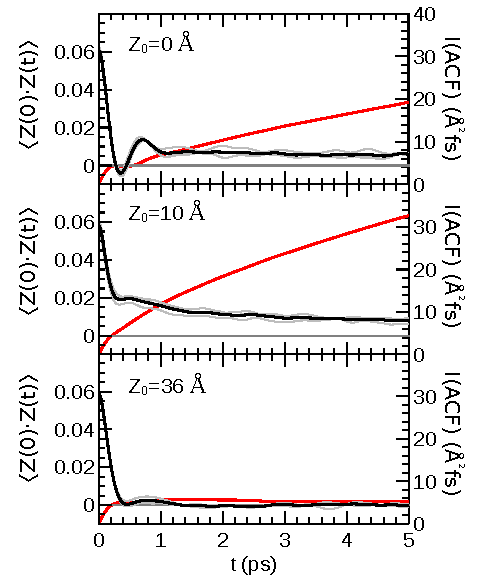
\includegraphics[width=0.65\textwidth]{Figures/acf-stacked}
    \caption{Time autocorrelation function of urea in the model DMPC bilayer 
    restrained at various values of $z_0$ using a harmonic potential 
    ($U_\mathrm{rest}=\frac{1}{2}k(z-z_0)^2$, $k=10$ kcal/(mol \AA$^2$)). 
    The black lines are the cumulative ACF calculated from three 1-ns simulations. 
    The ACF from each 1-ns trajectory alone is presented in grey. The red lines 
    (secondary axis) show the integral of the ACF over the interval $[0,t]$.}
    \label{fig:acf}
    \end{figure}

    \par Correlation functions typically require extensive sampling to achieve convergence, particularly for long correlation times. Heterogeneity of the bilayer environment can cause the ACF calculated from different simulations at the same $z$-reference value to be significantly discrepant, a particularly serious for hydrogen-bonding solutes that remain partially coordinated by water molecules inside the membrane such as urea (see Fig. S3). This issue can be addressed in part by performing several simulations, with a long equilibration period for each. The correlation functions can then be calculated from long time series, e.g., > 1 ns, collected from each of these simulations.

  \par The general features of the ACFs can be interpreted based on the analytical solution to the autocorrelation function of a harmonic oscillator undergoing Langevin dynamics,\cite{Tuckerman2010}
\begin{equation}
C_{zz}(t) = \textrm{var}(z) e^{-\gamma(\bar \omega)t/2\mu}[ \textrm{cos}(\Omega t) + \frac{\gamma(\bar \omega)}{2 \mu \Omega } \textrm{sin}(\Omega t)]
\label{eq:analytical-acf}
\end{equation}
   where $\gamma$ is the friction coefficient, $\bar \omega$ is the renormalized frequency of the oscillator, and $\mu$ is its reduced mass. $\gamma$ determines the rate of decay of the ACF. The expected behavior of the ACF based on Eq.~\ref{eq:analytical-acf} is that for damped periodic oscillations; however, if the friction coefficient, $\gamma$, is high, the ACF may decay to zero before there are any significant oscillations. This decay is apparent in the ACF when the solute is restrained at  $z=36$ \AA\ (bulk water; see Fig.~\ref{fig:acf}), which decays to zero within 0.5 ps, but then has a short second peak extending to 1.2 ps. The calculation of the diffusion coefficient formally requires the integration of the ACF in Eq.~\ref{eq:diff_hummer} over the interval $[0, \infty]$, but the ACF will  decay to zero within $\sim$ 2 ps in most fluid environments. Even if extensive sampling has been performed, there can be significant noise in the ACF at long times. Hummer noted that this noise causes the calculated diffusion coefficients to be sensitive to the interval of integration.\cite{Hummer2005} The g\_wham code~\cite{Hub2010}, one of the tools provided with Gromacs, limits the contribution of noise by cutting off the integration when the ACF drops below a threshold value of $0.05\ \times\ \textrm{var}(z)$.  This cutoff is not appropriate in all instances because the ACF can go through multiple oscillations before converging to zero. Nevertheless, it can provide reasonably accurate results if the autocorrelation function decays rapidly (i.e., in a high friction regime).

  \par Compared to bulk water, the autocorrelation functions in the lipid tail region are much slower to converge.  The ACFs from simulations with $z_0=10$ \AA\ and $z_0=0$ \AA\ only decay to 8 and 13\% of their initial values in 5 ps, respectively. A consequence of the 
failure to converge to zero is that the integrated ACF increases almost linearly, 
% what pateau?
%once the plateau is reached. This 
causing the calculated diffusion coefficients to be sensitive 
to the interval over which the ACF is integrated.  Typically, this sensitivity will cause 
the integrated ACF to be larger than it should be, so that the calculated diffusion coefficient is erroneously underestimated.

The slow convergence of the ACF is consistent with the work of Neale et al.,\cite{Neale2011} 
which showed that the convergence of US simulations of solute permeation 
into bilayers can require $\mu$s-ms-length simulations. Long correlation times are 
due to slow diffusion of the lipid tails, variations in the hydration of the solute, and
inhomogeneities in the bilayer interface that form over very long time scales.\cite{Neale2013}
While US simulations of the bilayer PMF can achieve convergence by running for a very long time, the 
lack of ergodicity in sampling is inconsistent with the underlying model of harmonic 
oscillator in frictional bath that is used to derive Eq.~\ref{eq:diff_hummer}.

The issues noted above for calculating diffusivity in the membrane are typically not 
significant for small solutes like water,\cite{Riahi2014,Issack2015} 
but they are severe for larger, more complex ones, such as urea, which are more prone to 
have long-time correlations. Under such circumstances, the Generalized Langevin method is not appropriate for 
calculating $D$($z$).  To determine if convergence issues are significant for a given 
system, the ACF should be calculated and plotted for several $z$-positions in the bilayer. If the ACF 
has not decayed to values near zero at long time scales (e.g., 5 ps), the Generalized Langevin 
method is probably not appropriate for calculating the position-dependent diffusivity for that solute. 

In the Generalized Langevin approach, a prerequisite noted above is that the force constant 
of the harmonic restraint should be sufficiently large to render the underlying free-energy 
surface a small perturbation on the harmonic potential.  The force constant used for the US 
simulations, 1.5\,kcal/mol/\AA$^2$, may be 
too small for application of this approach.  To test its applicability, we ran additional 
2-ns simulations for each window for urea using a much larger restraining force constant 
of 10\,kcal/mol/\AA$^2$.  However, as shown in Fig.~S6, the differences 
between the $D$($z$) profiles for the two cases are practically negligible at nearly all 
points.  At a few data points in the membrane interior, urea under a higher restraint 
gives a diffusivity as much as twice that of urea under a lower one.  Yet, because 
the permeability depends linearly on $D$($z$) (see Eq.~\ref{eq:solubility-diffusion}), but 
exponentially on $W$($z$), even a factor of two in the diffusivity across the entire permeation 
pathway contributes only $\sim$0.3 to log\perm.  Thus, for permeability calculations, it is 
acceptable to use the same simulations for calculation of both $W$($z$) and $D$($z$).

\subsection*{The Bayesian inference method}

%the accuracy of the approximation depends both on the strength
%of the confining potential and the magnitude of undulations
%in the intrinsic potential of mean force.

A fundamentally different approach for the determination of position-dependent 
diffusivities employs Bayesian inferences to reconcile thermodynamics and kinetics\cite{Hummer2005,Turkcan2012,Comer2013}.  This approach is especially suited for calculations within lipid membranes
because no assumptions are made regarding the form of the free-energy landscape on which diffusion occurs.
Furthermore, such an approach
is compatible with a wide variety of biasing schemes used in MD,
and thus, allows the practitioner more flexibility in simulation design.
This approach may be viewed as the
inverse solution of the Smoluchowski equation, which yields consistent estimates
of $W$($z$) and $D$($z$), given the
trajectory obtained from biased simulations.
These biases may also be time-dependent, as is the case for
the metadynamics and ABF algorithms.
Since the latter free-energy calculation algorithms are
designed for the accurate description of $W$($z$), one may use it as a
consistency check of the solution provided by the Bayesian inference method.
Alternatively, $W$($z$) as determined by a free-energy algorithm can
serve as a prior in the Bayesian scheme, increasing the reliability of
$D$($z$) in situations where statistics are poor.
In a nutshell, the Bayesian scheme uses as parameters the values of
the transition coordinate, $z$, along the trajectory, together with the force, $F(z,t)$,
which is the sum of the time-dependent bias and the intrinsic system force, equal
to $-\nabla W(z)$. Under the stringent assumption of a diffusive regime, the 
motion is propagated using a discretized Brownian integrator,
%
%% \begin{equation}
%% \label{Brownian}
%% \Delta z = z_2(t) - z_1(t) = \beta D(z_1) F(z_1, t_1) \Delta t + \nabla D(z_1) \Delta t + \sqrt{2 D(z_1) \Delta t} \ g(t) 
%% \end{equation}
\begin{equation}
 \Delta z = z_2(t) - z_1(t) = \beta D(z_1) F(z_1, t_1) \Delta t + \nabla D(z_1) \Delta t + \sqrt{2 D(z_1) \Delta t} \ g(t)
\label{Brownian}
\end{equation}
%
where $\beta = (k_B T)^{-1}$, $\Delta t = t_2 - t_1$ and $g(t)$
%is a Wiener process
%% (A Wiener process is an integral over Gaussian white noise, so the cumulative sum of many g(t))
is a Gaussian white noise of zero mean and variance equal to unity. Propagation along the
transition coordinate can be recast as the sum of a drift and a noise
term, i.e., $\Delta z = \mu + \sigma g(t)$, where
$\mu$ and $\sigma^2$, the variance, are defined by,
%
\begin{equation}
\left\{
\begin{array}{lcl}
\mu      & = & \beta D(z_1) F(z_1, t_1) \Delta t + \nabla D(z_1) \Delta t
\\
\sigma^2 & = & 2 D(z_1) \Delta t
\end{array}
\right.
\end{equation}
%
Propagation of motion obeys a Gaussian-distributed probability of observing the 
transition from $z_1$ at time $t_1$ to $z_2$ at time $t_2$,
%
\begin{equation}
\label{eq:Gaussian}
P[(z_2, t_2 | z_1, t_1) | F(z,t), D(z)] =
\frac{1}{\sigma \sqrt{ 2 \pi}}
\exp \left(-\frac{(\Delta z - \mu)^2}{2 \sigma^2} \right) 
\end{equation}
%
which assumes the system is in the overdamped Langevin dynamics regime and satisfies the 
fluctuation-dissipation theorem.
It is worth noting that in contrast with related
schemes, the present formalism, embodied in Eq.~\ref{Brownian}, features 
a gradient term, $\nabla D(z_1) \Delta t$, which has been shown to improve 
the accuracy of the predicted intrinsic system force, or gradient of the PMF.
%
See the SI for more details on applying the scheme 
to MD simulations.

As shown in Fig.~\ref{fig:acf}, the motion of permeants within the membrane is complex and correlations in such motion are much longer in the membrane environment than in solutions (at least several picoseconds).
These long correlation times complicate calculating the diffusivity by most
available methods, including the Bayesian inference method described herein.
A crucial component of this scheme is the time step, $\Delta t$.
%, which ought to be chosen with utmost care.
The correlations shown in Fig.~\ref{fig:acf} violate the assumptions of
overdamped Brownian motion leading to Eq.~\ref{Brownian}; thus, 
we found that $\Delta t$ values of a few picoseconds yield substantial overestimates of the diffusivity.
$\Delta t$ should be chosen to be much larger than any correlation
time of the motion; however, there is also an upper bound on $\Delta t$ because
the discretization implicit in Eq.~\ref{Brownian} requires
only small changes in $F(z_1, t_1)$ and $D$($z$) over the duration of $\Delta t$.
Errors due to the violation of this requirement are apparent when
$W$($z$) as predicted by the Bayesian scheme diverges substantially
from that obtained by the free-energy calculation technique
(here, ABF).
%We are currently developing an improved scheme to 
%remove the restrictions imposed by discretization. 
For the permeants examined in the present work,
we found $\Delta t=32$~ps still gives consistent $W$($z$)
functions while minimizing errors due to correlation.

\subsection*{Comparison of the two approaches}
As is clear from Eq.~\ref{eq:solubility-diffusion}, log\perm~is much more sensitive to $W(z)$ than to $D$($z$).
However, as shown in Fig.~\ref{fig:Dz}, there are some notable differences
in the results of the Generalized Langevin and Bayesian inference approaches, which
have an appreciable effect on the predicted permeability.
For the four methods used to determine the PMF, the Generalized Langevin approach 
for calculating $D$($z$) was used for US and REUS, while the Bayesian inference method 
was used for ABF and MW-ABF.
Under the conditions described above, i.e. the restraint strength used in the US and REUS
simulations and the $\Delta t$ chosen for the Bayesian scheme,
we obtain smaller diffusivity values using
the Generalized Langevin approach than using the Bayesian approach.
These differences are most notable near $z=0$, where the value of $D$($z$)
most influences the permeability for urea due to the maximum of $W$($z$).
For example, the much larger diffusivity of urea
near the center of the membrane as determined by the Bayesian scheme
compared to the Generalized Langevin scheme (see Fig.~\ref{fig:Dz}) 
results in the ABF and MW-ABF methods having larger log\perm~values by more than
an order of magnitude, despite the fact that the
height of the free energy barrier calculated by ABF is significantly
larger than that for the other methods (see Fig.~\ref{fig:PMFs}).
{\color{red} The generally larger $D(z)$ values given by 
the Bayesian scheme are likely due to the fact that
the scheme used in the present work is limited to relatively small values of $\Delta t$, a consequence of the Gaussian approximation for the probability profile (Eq.~\ref{eq:Gaussian}). We have found that the motion of the permeants is not strictly diffusive at the $\Delta t$ values used here and that the diffusivity appears to decrease continuously with $\Delta t$. We are currently working to improve the Bayesian scheme to overcome the limitations on $\Delta t$, which will be addressed in subsequent work.}
Hence, although it plays a less dramatic role in Eq.~\ref{eq:solubility-diffusion} than $W$($z$),
$D$($z$) is also highly influential and the approach to calculating it must be
carefully considered.


%Despite the vast differences between the two methods, 
%they produce similar results, shown in Fig.~\ref{fig:Dz} for all three permeants.  


\begin{figure}[htbp]
\begin{center}
	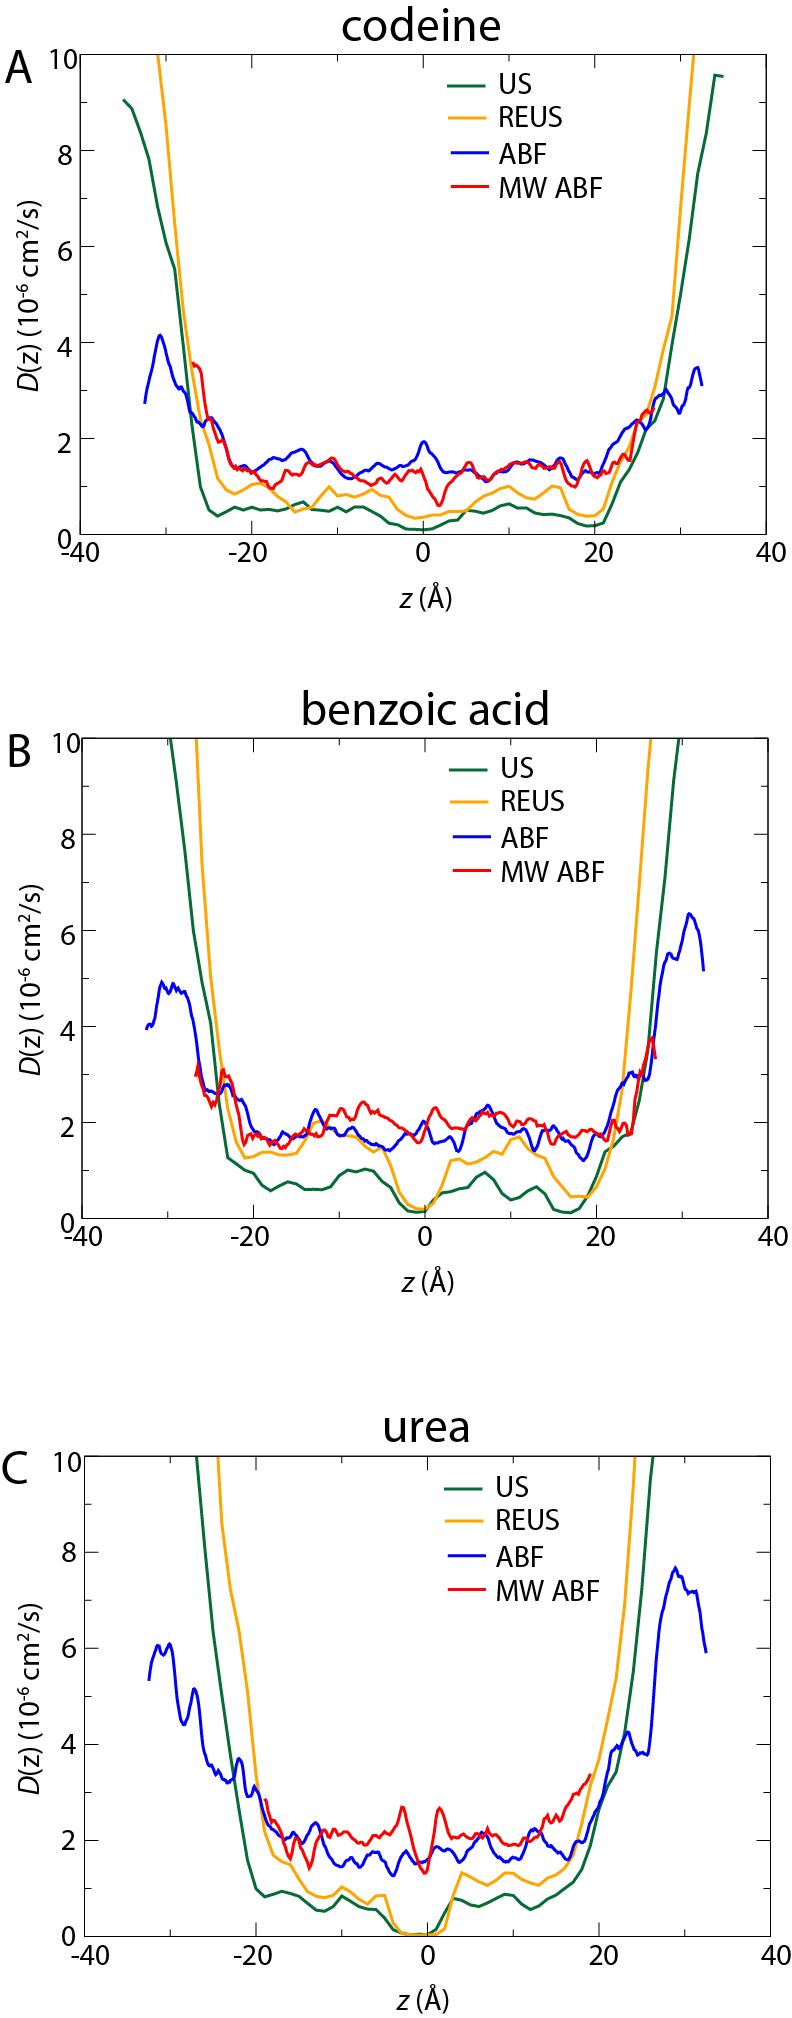
\includegraphics[width=0.4\textwidth]{Figures/Dz-all}
	\caption{Diffusivity profiles for each permeant, (A) codeine, (B) benzoic acid, and (C) urea.  In green and orange are the umbrella-based methods, US and REUS, for which the Generalized Langevin approach was used to determine $D$($z$).  In blue and red are the ABF-based methods, for which the Bayesian scheme was used.}
	\label{fig:Dz}
\end{center}
\end{figure}




% moved from end of last section



%Section: "Comparison of the methods"  (JC)
%       -rate of convergence of PMFs
%       -each method's Dz with same PMF (no)
%       -each method's PMF with same Dz (no)
%       -does any method stand out?
%
%    Section: Error tolerance and robustness (Conner)
%       -modeling PMFs / D(z) using simple functions and limited data (e.g., just a couple of points along the curve)
%       -range of logP$_m$s obtained depending on uncertainty

\section*{Comparison of methods and tolerance to error}
  \par Results presented up to this point do not favor any one method over another.  For example, while REMD-US is more accurate for urea, it is less so for the other two permeants (see Table~\ref{table:results}).  To examine if the rate of convergence depends on the method employed, we have plotted for each method and permeant log\perm~as a function of simulation time in Fig.~\ref{fig:deltaP}.  For codeine and benzoic acid, the variance in log\perm~for a given method is quite small, no more than 0.25 log units, even between 360\,ns and almost 3\,$\mu$s, suggesting that as much as 90\% of the simulation time invested was unnecessary.  On the other hand, there is a clear effect of time on log\perm~for urea, with it changing by as much as two log units over time.   The downward trend for urea's log\perm~is an effect of the shrinking peak in the PMF (Fig.~\ref{fig:PMFs}C).   A similar trend for codeine or benzoic acid is likely not observed because the peaks in their PMFs, i.e., those parts above 0 that contribute most significantly to log\perm, are almost non-existent.   Regardless, for codeine and benzoic acid, the disagreement with experiment is notable in part because the simulated values are consistently greater by 0.5 to 1.5 log units.

%\begin{figure}[htbp]
%\begin{center}
%	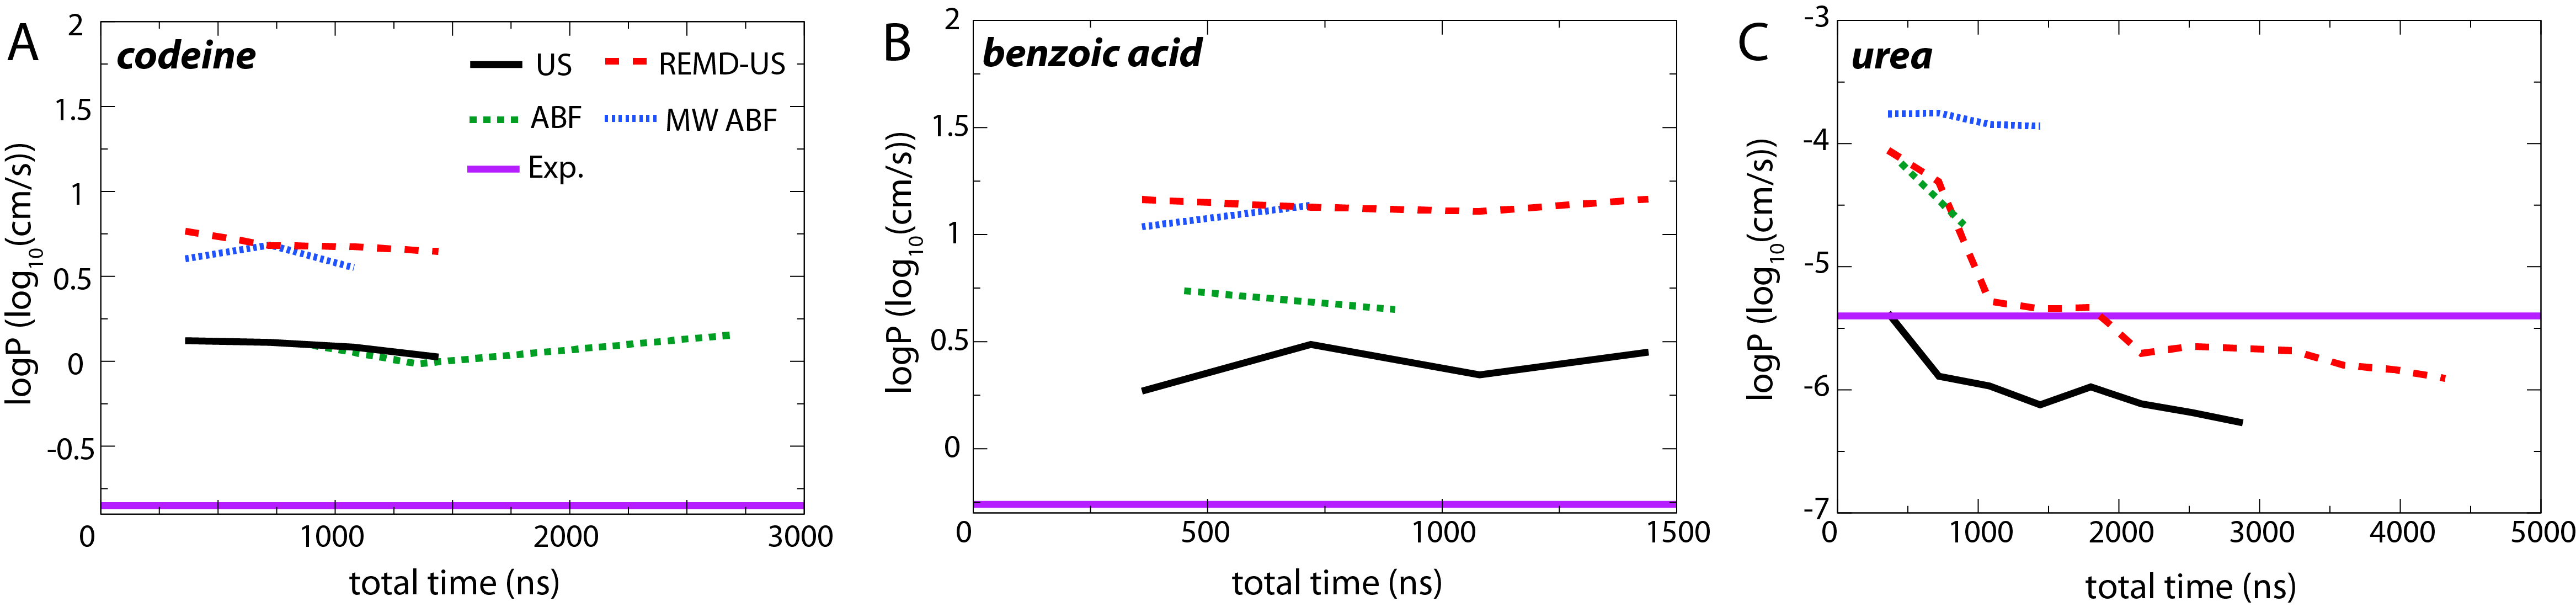
\includegraphics[width=0.9\textwidth]{Figures/converge}
%	\caption{Convergence of log\perm~for the three permeants, (A) codeine, (B) benzoic acid, and (C) urea.  Experimental values are shown as solid purple lines, with those from the simulations as indicated in the legend.}
%	\label{fig:converge}
%\end{center}
%\end{figure}

%\section*{Error tolerance}

  \par After examining the PMFs and diffusivities in great detail, it is useful to consider their individual contributions to the permeability and, thus, how accurate each of them ought to be to give log\perm~at a chosen level of accuracy.  To explore how these two parameters contribute to the permeability, a program to generate arbitrary PMFs and diffusivities was written.  This program creates smooth profiles based on input values of the PMF and diffusivity at the interfacial region and at the center of the membrane (see Methods for more details).  We first used the program to test molecules with a single barrier (or valley) at the membrane center, varying the barrier's height and width.  As seen in Fig.~\ref{fig:models}A, the contribution of the width is negligible, while the height of the barrier dominates log\perm.  For positive PMF values 
  %greater than 0\,kcal/mol 
 at the center, there is roughly a correspondence of 2\,kcal/mol to one log unit for log\perm.  Changing the diffusivity by a factor of 10 (range of $10^{-6}$ to $10^{-5}$\,cm$^2$/s) has a similar effect of one log unit, as expected from the linear dependence of the permeability on $D$($z$) (see Fig.~\ref{fig:models}B).  Nearly identical behavior was observed when two barriers were placed at the interfacial region, with only the height and not the position of the barriers contributing (see Fig.~S7).

\begin{figure}[htbp]
\begin{center}
	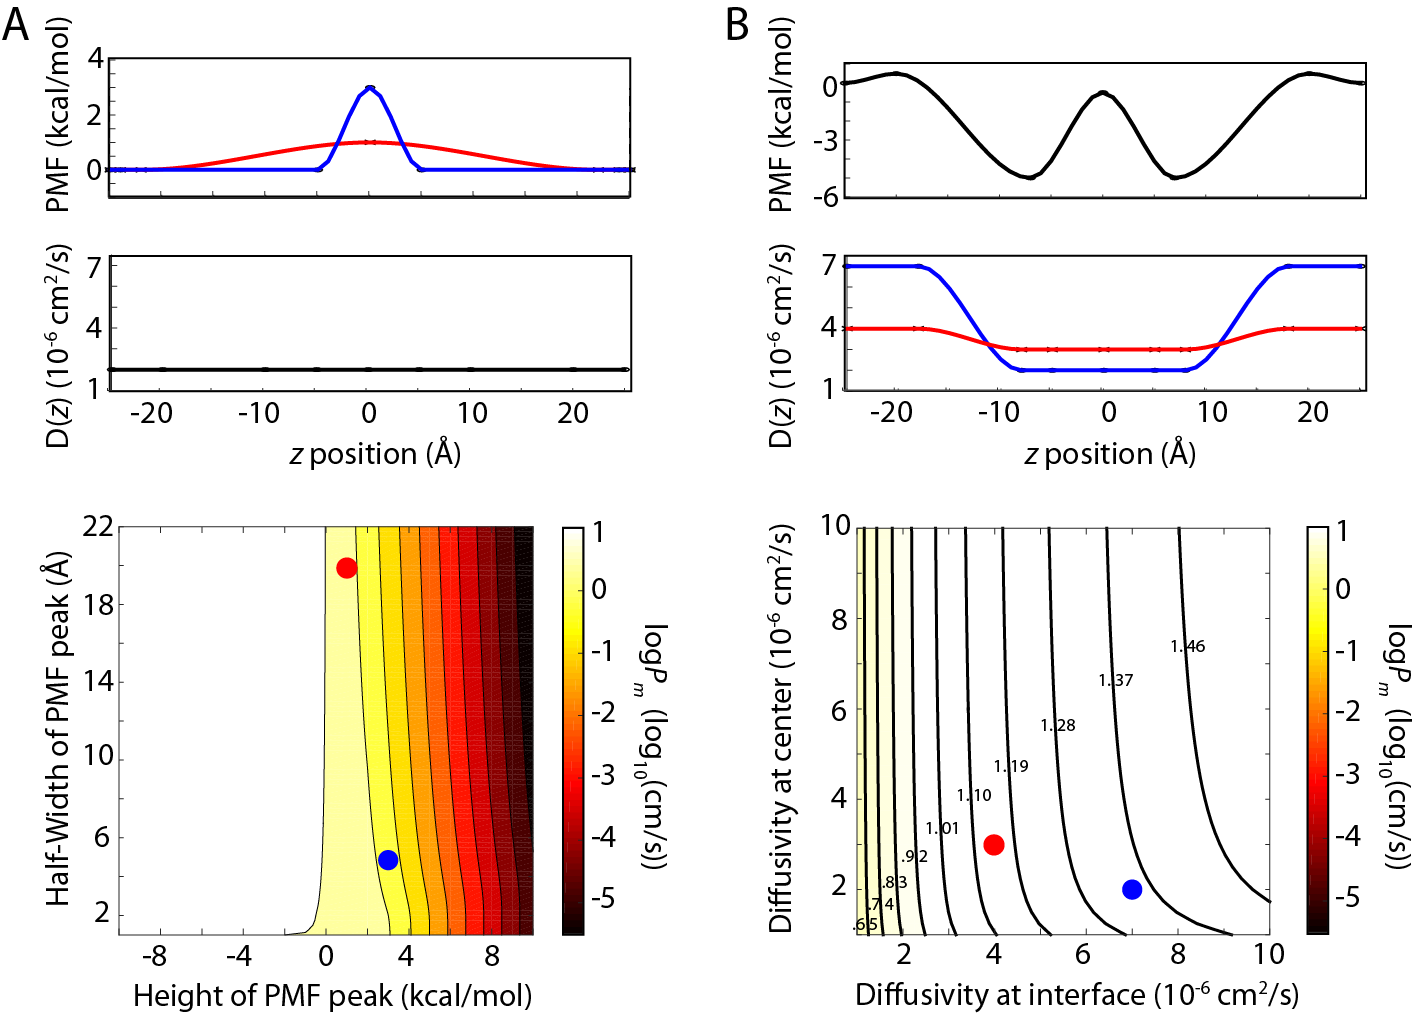
\includegraphics[width=0.9\textwidth]{Figures/models}
	\caption{log\perm~as a function of modeled input.  In both parts, the input PMF and $D$($z$) are shown on top and the dependence of log\perm~on them on bottom.  In each contour plot, the red and blue circles correspond to the red and blue PMF or diffusivity above.  (A) log\perm~as a function of PMF barrier height and width.  $D$($z$) is held constant.  (B) log\perm~as a function of diffusivity profile.  The PMF is held constant.  $D$($z$) is varied at $z=\pm 20$\,\AA~(interface) and at $z=0$\,\AA~(center).  The range of log\perm~values is 0.55 to 1.55, with contour values given in the figure.}
	\label{fig:models}
\end{center}
\end{figure}

  \par While permeants for which the PMF barrier is pronounced have their log\perm~values dominated by the barrier height, others may exhibit more subtle dependencies.  To test this possibility, a PMF in which the barriers are less than 1\,kcal/mol at the interfacial regions of the membrane, akin to the PMFs for codeine or benzoic acid, was created and the diffusivity profile varied.  As shown in Fig.~\ref{fig:models}B, the diffusivity at the PMF barriers contributes to log\perm, but that at the core (a minimum in the PMF) does not.  As a final test of the minimal amount of information necessary to calculate log\perm, we generated PMFs and diffusivities to match those from simulation based solely on the PMF value at the peak(s) and $D$($z$) at that position.  Comparison of each generated profile to the computed ones is presented in Fig.~S8.  The obtained log\perm~values are 0.31 (benzoic acid), 0.44 (codeine), and $-5.82$ (urea).  While urea is identical to the value estimated with REUS (see Table~\ref{table:results}), the other two permeants are slightly below their computed values (difference of 0.85 and 0.63, respectively), although they are closer to experimental values.  Regardless, our models demonstrate that log\perm~can be obtained from surprisingly few data points to a high degree of accuracy.

%Even so, an order of magnitude change in the diffusivity only changes the log\perm~by 1 log unit, as would be expected from the functional dependence in Eq.~\ref{eq:xx}.

%The net result of the idealized profiles is that a calculation of log\perm~is dominated by, first and foremost, the PMF maximum.  Indeed, if precision to within one log unit is all that is required, the maximum of the PMF is sufficient.  Further precision can be obtained by knowing the diffusivity at the maximum.  As evidence of this point, we determined log\perm~for each permeant using our program and only the location(s) and value(s) of the PMFs at their maxima.  ... (to do)

%Because the solubility-diffusion model relies on two position-dependent quantities, the PMF and diffusivity, it is natural to assume they must be calculated to determine the permeability.  However, as demonstrated in the section ``Comparison of methods and tolerance to error'', only a few data points contribute significantly to it.  Therefore,
  \par In lieu of determining the full PMF, which can require microseconds of simulation, one can use alternative methods to sample the critical points, i.e., at the interface and/or at the center.  As a proof-of-concept, we ran alchemical free energy perturbation (FEP) to calculate the solvation free energy of urea in the membrane core and in water.  We found $\Delta G = 9.26$\,kcal/mol ($\sim$1--1.5\,kcal/mol higher than predicted by our PMFs in Fig.~\ref{fig:PMFs}) and $D(0) = 1.25\times 10^{-6}$\,cm$^2$/s.  When combined with a very simple interpolated PMF curve that goes smoothly to 0 at $z=\pm20$\,\AA, we find log\perm = $-5.26$.  This is within < 3\% of the experimental value, despite requiring significantly less simulation time: 200\,ns for FEP vs. at least 1\,$\mu$s for the full-PMF approach.  However, one loses insight into the details of the permeation process when using FEP over a PMF-based method.


%Thus, we recommend that sampling be focused on critical regions where barriers are expected, e.g., the membrane core and/or interfacial region.

% Conclusions  (JC?)
%  *difficulties that arise in the calculations - slow membrane reorganization, solute reorientation, etc.  (here and/or maybe intro?)
%  *what method to use, when, how to prepare?
%  *where best to invest limited computational time? 
%  *how much sampling is really needed to get within a certain error?  (e.g., +/- 1 log unit)
%  *take home message: can MD ever be used to reliably predict permeabilities?  
%   -is there a way to streamline the process for high throughput calculations?
%

\section*{Conclusions}

We have computed the membrane permeability to three compounds using a variety of simulation-based methods, namely US and ABF, along with their multiple-copy variants, REUS and MW-ABF, respectively.  These three compounds, codeine, benzoic acid, and urea, span a range of chemical properties and, most importantly, permeabilities (see Table~\ref{table:results}).  All simulation methods were able to predict the permeability within one log unit typically, except in a few cases that were off by 1.5 (see Fig.~\ref{fig:deltaP}).  Interestingly, of the four methods tested, none stood out as unequivocally better than the others.  The root-mean-square error in log units for each method was 0.821 (US), 1.23 (REUS), 1.33 (ABF), and 1.08 (MW-ABF). 

Because of their similar performances, no one simulation method is recommended over another.  However, regardless of the method chosen, certain procedures can improve convergence.   It was found that simulation over the entire range, i.e., from one side of the membrane to the other, followed by symmetrization of the resulting PMF converged much faster than simulating over just half the range, i.e., from one side to the membrane center (see Fig.~S5).  Additionally, the states used to seed the windows for production sampling should be well equilibrated.  Methods such as SMD used to produce these initial states induce significant non-equilibrium perturbations to the membrane that may take hundreds of nanoseconds or more to equilibrate.  Alternatives to SMD include building the membrane {\it de novo} around the permeant at varying depths~\cite{Dorairaj2007} or introducing the permeant in a perturbative fashion at different values of $z$.  Regardless of the method, equilibration should be carried out for as long as is feasible (50-100\,ns/window at least, depending on membrane depth), particularly when the permeant's stability relies upon the spontaneous formation of membrane defects and penetration of water.

Two methods for calculating the diffusivity were explored.  The first, more commonly used Generalized Langevin method, based on restraining the solute and measuring the correlation of the system forces acting on it, was combined with the PMFs in the US and REUS; the second, the Bayesian inference method, was combined with PMFs from ABF and MW-ABF.  Both methods present a number of subtleties that prevent a straightforward calculation of $D$($z$), e.g., a proper choice of the force constant in the Generalized Langevin method or the discretization time step in Bayesian inference.  Furthermore, they are both plagued by long correlation times that are not amenable to the usual MD time scales.  Despite these caveats, they produced diffusivity profiles in rough agreement, although those from the Bayesian inference method are consistently slightly higher in the membrane than those from the Generalized Langevin method (see Fig.~\ref{fig:Dz}).  

Because the solubility-diffusion model relies on two position-dependent quantities, the PMF and the diffusivity, it is natural to assume they must be calculated to determine the permeability.  However, as demonstrated in the section ``Comparison of methods and tolerance to error'', only a few data points contribute significantly to it.  Therefore, permeability can be estimated from a handful of parameters, namely the values of $W$($z$) and $D$($z$) at the membrane/water interface and at the membrane center, with the remainder interpolated from an expected smooth topology.  Going even further, extrapolating from just a single value each of the PMF and the diffusivity at the membrane center for urea (see Fig.~\ref{fig:models}A) produced a log\perm~almost identical to the experimental value.  Thus, we recommend that sampling be focused on critical regions where barriers are expected, e.g., the membrane core and/or interfacial region.

Taken together, the results show the robustness of a variety of MD-based methods in calculating membrane permeability for small molecules.  In particular, all methods {\color{red} appear to} converge on sub-$\mu$s time scales, although the determined log\perm~values are nearly all 0.5 to 1.5 log units above the experimental values.  This consistent overestimation is in agreement with a previous MD study from 2004~\cite{Bemporad2004}, despite using 10-100$\times$ longer simulations in the current study.  {\color{red} The membranes compared, DMPC in simulation with egg PC in experiment, are not identical, which may contribute to the discrepancy.}  Another possible reason could be slow membrane reorganization that occurs on a time scale even an additional 2-3 orders of magnitude greater~\cite{Neale2011}.  The lack of polarizability is another tempting possibility, given the vastly different environments experienced by the permeating molecule~\cite{Riahi2014}.  
Similarly, the most commonly used force fields (including CGenFF used in this study) are primarily parameterized to reproduce phenomena obtained in aqueous environments. Thus, it may be unrealistic to expect that solute phenomena within the non-polar membrane environment is as well represented. Therefore, further exploration of the force-field effects within lipid-like or non-polar environments are warranted.  In particular, inclusion of explicit polarizability may improve accuracy, although at a computational cost of 2-6$\times$~\cite{Chowdhary2013,Wang2013}.  {\color{red} However, given the lack of convergence of the four methods to a single value for each permeant, all of which use the same force field, it cannot be known a priori to what degree, if any, changes to the force field will improve agreement with experiment.}
Additionally, the assumptions of the solubility-diffusion model, such as the reliance on a single reaction coordinate and that permeation obeys classical diffusion, may need to be challenged to obtain improved quantitative agreement with experimental measures~\cite{Orsi2010,Parisio2013,Comer2014}.

Finally, we draw attention to the potential benefit of our results to QSPR models.   
%Even if the explicit-membrane permeability calculations reported here were perfectly accurate, they are still too computationally demanding to replace QSPR, taking weeks where results are needed in less than a day.  However, 
We have shown that only one or two points in the PMF and diffusivity contribute significantly to the permeability.  Thus, calculations for a single permeant focusing on these critical points could be done in hours on a sufficiently fast cluster.  Furthermore, the location of these points, typically at the membrane center or at the water/membrane interface, suggest reduced systems that could represent them reasonably well, e.g., octanol for the interfacial region.  
Combined with improved force fields, fast calculations on such reduced systems could augment the molecular descriptors used to design QSPR models, similar to the ``membrane-interaction QSAR'' approach pioneered by Hopfinger et al.~\cite{Kulkarni1999,Tseng2012}.




%!TEX root = bcd_SI.tex

\section*{Methods}
\subsection*{System Preparation} 
\par GAFF\cite{Wang2004,Wang2006} forcefield parameters for the seven guest molecule
along with both GAFF and Q4MD-CD\cite{Cezard2011} parameterizations of $\beta$-cyclodextrin 
were obtained from Tang and Chang\cite{Tang2017}. For comparison we use identical structure and
parameterizations as those used in their study. These initial structures were 
used by the SEEKR software for preparation of the milestoning simulations. 
The preparation procedure was the same for each of the seven guest molecules and 
followed standard SEEKR protocols\cite{Votapka2017}. All systems were solvated 
with TIP3P waters\cite{Jorgensen1983a}.

\subsubsection*{Preparation of milestoning simulations with SEEKR} 
\par The bound state of the host-guest complex was defined as the center of mass (COM) 
of the \bcd. The guest molecule was considered to be bound when 
its COM was within 1.5~\AA of the bound state coordinates. From this bound state, 
spherical milestones were defined in increasing 1.5~\AA increments from 1.5~\AA to
13.5~\AA. Furthermore, spherical milestones of radius 7.5~\AA and less, were 
divided into two half-spheres to better capture the asymmetries between the two faces. 
When the ligand is less than 7.5~\AA away from the bound state, it is trapped on 
a particular face due to the size of the host molecule. For milestone distances 
greater than 7.5~\AA, the ligand was found to freely sample both faces, and therefore 
a single spherical milestone was sufficient for sampling host-guest interactions. 
In total, 14 unique milestones were defined. In practice, this was achieved via 
post-processing the simulations on each face to identify any trajectories that 
crossed from one face to the other, and modifying the transitions accordingly in 
the milestoning model. In addition, two simulations were conducted for the outermost 
milestones (one with the ligand initiated on each face), and these were then 
combined into a single milestone (with double the sampling) for milestones that 
were not restricted to a particular face.


\par The first 13 milestones correspond to the MD region, while the 14th and 
outermost milestone corresponds to the BD region. The standard SEEKR preparation 
protocol\cite{Votapka2017} was then used to generate the coordinate, parameter, 
and simulation files necessary for a milestoning calculation. For each of the MD 
milestones, a copy of the apo \bcd structure was generated and the guest 
molecule was then placed at the appropriate radius from the bound state coordinates. 
Any water molecules that clashed with the guest molecule were removed. The guest 
distribution for the BD milestone was constructed by first running a conventional 
BD simulation where trajectories terminated at the appropriate distance for the 
milestone surface (13.5~\AA).

\subsection*{Simulation}
\subsubsection*{MD Simulations}
\par A modified version of NAMD 2.12 was used for all MD simulations\cite{Phillips2005}.
For all 13 milestones in the MD region, the standard SEEKR procedure for 
minimization, equilibration and simulation was followed. First, 5000 steps of 
minimization were performed to allow for relaxation, particularly of solvent, 
around the newly placed guest molecule. Further relaxation of the solvent was 
achieved by a series of 2~ps heating simulations that gradually increased the 
temperature from 298~K to 350~K and then cooled back to 298~K. Host and guest atoms 
were constrained during these heating simulations to ensure that the guest 
remained on the appropriate milestone surface. To obtain the equilibrium 
distribution of the guest molecule on each milestone, 200 ns of constant 
volume simulation was performed. A $\SI{90}{kcal\cdot mol^{-1}\cdot\angstrom^{-2}}$ 
harmonic restraint was used to hold the COM of the guest molecule at the appropriate 
distance from the binding site. To minimize any bias of the arbitrary guest 
starting conformation, the first 40~ns of each simulation were discarded and 
therefore were not included as part of the equilibrium distribution. From these 
trajectories, position and velocity configurations were selected every 0.2~ns, 
resulting in a total of 800 configurations per milestone. To obtain the first
hitting point distribution (FHPD) of each milestone, 10 independent and 
unrestrained simulations were initiated from these equilibrium configurations. 
Each simulation was propagated backwards in time by reversing its velocity at 
constant energy and volume (a total of 8000 reversals for each milestone). 
Only trajectories that struck an adjacent milestone before recrossing the 
milestone on which they originated were included as part of the FHPD for that 
milestone. To obtain the transition probabilities and times necessary for the 
calculation of kinetic parameters, all members of the FHPD were brought back to 
their starting position and velocity and new unrestrained simulations were then 
initiated from each configuration. These simulations were propagated forward in 
time at constant energy and volume. Once a simulation crossed its starting 
milestone again, it was monitored for crossing of adjacent milestones. 
When an adjacent milestone was crossed, the simulation was stopped and the 
transition and incubation time were recorded. Although more of the equilibrium 
simulation trajectories could likely have been used without biasing the results 
based on the starting conformation, the 8000 reversal trajectories that resulted 
from the 160~ns used were more than sufficient to sample the transitions between 
the milestones, resulting in hundreds of observed transitions between each milestone. 
In total, 2.6~${\mu}s$ of equilibrium sampling (160~ns for 16 milestones) were 
used and approximately 570~ns of FHPD sampling for a total of 3.2~${\mu}s$ of 
simulation used in the milestoning model. The total cost per ligand (including 
simulation discarded for equilibration) was therefore $\sim$3.8 ${\mu}s$. 
 %This is roughly half of the simulation time needed by Tang and Chang.

\subsubsection*{BD Simulations}
\par All BD simulations were performed using the BrownDye software package\cite{Huber2010}. 
Electrostatic potentials of the host and guest molecules used as inputs for the 
BD simulation were calculated with APBS version 1.4\cite{Baker2001}. To match 
experimental conditions, APBS calculations and BD simulations were carried out 
with a solvent dielectric of 78, a solute dielectric of 2, and zero ionic concentration. 
An initial series of simulations were initiated from the b-surface, a sphere that 
encloses the entire host molecule and has sufficient radius for the guest molecule 
to be situated in bulk solvent such that forces between the host and guest are centrosymmetric. 
$10^6$ independent BD simulations were initiated from random points on the b-surface 
and and were propagated until the guest either contacted the outermost milestone 
(13.5~\AA) or escaped. Trajectories that successfully contacted the 13.5~\AA milestone 
were used as the FHPD for this milestone. Another series of $10^6$ BD simulations 
were initiated from the FHPD and propagated until contacting the second-outermost 
milestone (12.0~\AA) or escaping to the q-surface. This procedure is automated by 
SEEKR.

\subsection*{Milestoning Calculations}
\par Statistics from all milestones in the MD and BD regions were extracted 
using SEEKR and combined to construct a transition kernel as well as an incubation 
time vector. These are the two key quantities for the calculation of kinetic 
parameters in milestoning theory.\cite{Faradjian2004} As described previously, 
a post-simulation analysis was performed to account for ligand transitions 
between the two faces of the \bcd ring for milestones of radius 7.5~\AA 
or less. The analysis portion of SEEKR was then used to compute the desired 
kinetic quantities, \kon and \koff, as well as the free energy of binding $\Delta G_{bind}$.


\section*{Supporting Information}
Theoretical details of application of the Bayesian scheme to MD, analysis of membrane structure from MD simulations. This information is available free of charge via the Internet at http://pubs.acs.org/.

\section*{Acknowledgements}
CTL acknowledges support from the NIH Molecular Biophysics Training Program (T32-GM008326).  JC was supported by Kansas Bioscience Authority funds to the Institute of Computational Comparative Medicine (ICCM) at Kansas State University and to the Nanotechnology Innovation Center of Kansas State University (NICKS).  JCG acknowledges a CAREER award from the National Science Foundation (MCB-1452464), a Burroughs Wellcome Fund Collaborative Research Travel Grant and supercomputing resources provided by the National Institute for Computational Sciences at Oak Ridge National Lab through the Extreme Science and Engineering Discovery Environment (XSEDE), supported by NSF grant number OCI-1053575.  CNR thanks NSERC of Canada for funding through the Discovery Grant program (Application 418505-2012) and Compute Canada (RAPI: djk-615-ab) for supercomputing resources.  YW acknowledges Project 21403183 supported by National Natural Science Foundation of China.  REA acknowledges a NIH Director's New Innovator Award DP2 OD007237, the National Biomedical Computation Resource (NBCR) NIH P41 GM103426, and supercomputing resources provided by XSEDE (NSF TG-CHE060073).  REA is a co-founder of Actavalon, Inc.
